\documentclass{article}
\usepackage{setspace}
\usepackage{listings}
\usepackage{color}
\usepackage{amsmath}
\usepackage{amssymb}
\usepackage{amsthm}
\usepackage{graphicx} 
\usepackage{float} 
\usepackage{fancyhdr}                                
\usepackage{lastpage}                                           
\usepackage{layout}   
\usepackage{subfigure} 
\definecolor{codegreen}{rgb}{0,0.6,0}
\definecolor{codegray}{rgb}{0.5,0.5,0.5}
\definecolor{codepurple}{rgb}{0.58,0,0.82}
\definecolor{backcolour}{rgb}{0.95,0.95,0.92}

\lstdefinestyle{mystyle}{
    backgroundcolor=\color{backcolour},   
    commentstyle=\color{codegreen},
    keywordstyle=\color{magenta},
    numberstyle=\tiny\color{codegray},
    stringstyle=\color{codepurple},
    basicstyle=\footnotesize,
    breakatwhitespace=false,         
    breaklines=true,                 
    captionpos=b,                    
    keepspaces=true,                 
    numbers=left,                    
    numbersep=5pt,                  
    showspaces=false,                
    showstringspaces=false,
    showtabs=false,                  
    tabsize=2
}
\pagestyle{fancy}  
\lhead{ZHANG HUAKANG}
\chead{Assignment 7} 
\rhead{DB92760} 
\renewcommand{\baselinestretch}{1.05}
\title{Assignment 7 of CISC 2002}
\author{ZHANG Huakang/DB92760}

\begin{document}
    \maketitle
    \section{}
        \subsection{}
        \paragraph{}
            \lstinputlisting[language=Matlab,style=mystyle,caption=Code ]{code/Assignment_7_1_x.m}
            \lstinputlisting[language=Matlab,style=mystyle,caption=Code ]{code/Assignment_7_1_f.m}
            \lstinputlisting[language=Matlab,style=mystyle,caption=Code ]{code/Assignment_7_1_1.m}
            \lstinputlisting[language=Matlab,style=mystyle,caption=Code ]{code/Assignment_7_1_1output}
        \subsection{}
            \paragraph{}
            \lstinputlisting[language=Matlab,style=mystyle,caption=Code ]{code/Assignment_7_1_2.m}
            \lstinputlisting[language=Matlab,style=mystyle,caption=Code ]{code/Assignment_7_1_2output}
        \subsection{}
            \paragraph{}
            \lstinputlisting[language=Matlab,style=mystyle,caption=Code ]{code/Assignment_7_1_3.m}
            \lstinputlisting[language=Matlab,style=mystyle,caption=Code ]{code/Assignment_7_1_3output}
        \subsection{}
        \paragraph{}
            \lstinputlisting[language=Matlab,style=mystyle,caption=Code ]{code/Assignment_7_1_4.m}
            \lstinputlisting[language=Matlab,style=mystyle,caption=Code ]{code/Assignment_7_1_4output}
            \begin{figure}[H] 
                \centering 
                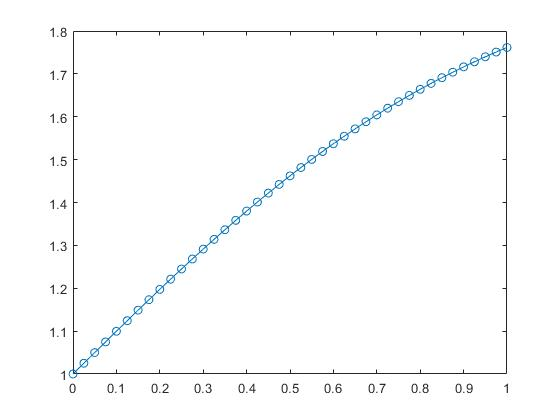
\includegraphics[width=0.9\textwidth]{img/Assignement_7_1.jpg}
                \caption{Figure} 
            \end{figure}
    \section{}
        \subsection{}
            \paragraph{}
            Let $\frac{dx}{dt}=x_1$
            \begin{equation*}
                \begin{split}
                    x(0)=&0\\
                    \frac{dx}{dt}(0)=&-1\\
                    x_1(t)=&\frac{dx}{dt}\\
                    \frac{dx_1}{dt}(t)=&-x
                \end{split}
            \end{equation*}
        \subsection{}
            \begin{equation*}
                \begin{split}
                    x_{n+1}=&x_{n}+\Delta t x_1(t_n,y_{1n},y_{2n})\\
                        =&x_{n}+\Delta t x_1(t_n)\\
                    x_{1n+1}=&x_{1n}+\Delta t (-x_n)\\
                \end{split}
            \end{equation*}
            $$\Delta t=\frac{\pi}{10}$$
            \begin{equation*}
                \begin{split}
                    x_{11}=&x_{10}+\Delta t (-x_0)\\
                        =&-1+\frac{\pi}{10}(-0)\\
                        =&-1\\
                    x_1=&x_0+\Delta t x_{11}\\
                        =&-\frac{\pi}{10}\\
                    x_{12}=&x_{11}+\Delta t (-x_1)\\
                        =&-1+\frac{\pi^2}{100}\\
                    x_2=&x_1+\Delta t x_{12}\\
                        =&-\frac{\pi}{5}+\frac{\pi^3}{1000}\\
                    x_{13}=&x_{12}+\Delta t(-x_2)\\
                        =&-1+\frac{\pi^2}{100}+\frac{\pi}{10}(\frac{\pi}{5}-\frac{\pi^3}{1000})\\
                        =&-1+\frac{3\pi^2}{100}-\frac{\pi^4}{1000}\\
                    x_3=&x_2+\Delta t x_{13}\\
                        =&-\frac{\pi}{5}+\frac{\pi^3}{1000}+\frac{\pi}{10}(-1+\frac{3\pi^2}{100}-\frac{\pi^4}{1000})\\
                        &...\\
                    x_5\approx &-1.0125\\
                \end{split}
            \end{equation*}
            \lstinputlisting[language=Matlab,style=mystyle,caption=Code ]{code/Assignment_7_2_1.m}
            \lstinputlisting[language=Matlab,style=mystyle,caption=Code ]{code/Assignment_7_2_1output}
        \subsection{}
            \begin{equation*}
                \begin{split}
                    k_1=&\Delta t x_1(t_n)\\
                    l_1=&\Delta t -x\\
                    k_2=&\Delta t x_1(t_n+k1)\\
                    l2=&\Delta t -(x+l2)\\
                    x_{n+1}=&x_n+\frac{1}{2}(k_1+k_2)\\
                    x_{1n+1}=&x_{1n}+\frac{1}{2}(l_1+l_2)\\
                \end{split}
            \end{equation*}
        \subsection{}
            \begin{equation*}
                \begin{split}
                    k_1=&\Delta t x_1(t_n)\\
                    l_1=&\Delta t -x\\
                    k_2=&\Delta t x_1(t_n+\frac{1}{2}\Delta t)\\
                    l_2=&\Delta t -(x+\frac{1}{2}k_2)\\
                    k_3=&\Delta t x_1(t_n+\frac{1}{2}\Delta t)\\
                    l_3=&\Delta t -(x+\frac{1}{2}k_3)\\
                    k_4=&\Delta t x_1(t_n+k3)\\
                    l4=&\Delta t -(x+l3)\\
                    x_{n+1}=&x_n+\frac{1}{6}(k_1+2k_2+2k_3+k_4)\\
                    x_{1n+1}=&x_{1n}+\frac{1}{6}(l_1+2l_2+2l_3+l_4)\\
                \end{split}
            \end{equation*}
        \subsection{}
            \lstinputlisting[language=Matlab,style=mystyle,caption=Code ]{code/Assignment_7_2_3.m}
            \begin{figure}[H] 
                \centering 
                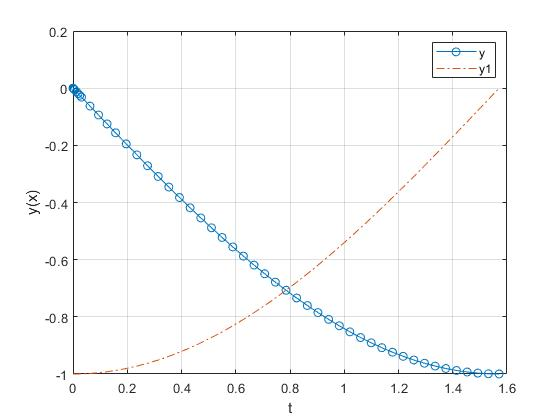
\includegraphics[width=0.9\textwidth]{img/Assignement_7_2.jpg}
                \caption{Figure} 
            \end{figure}
    \section{}
        \subsection{}
            \lstinputlisting[language=Matlab,style=mystyle,caption=Code ]{code/Assignment_7_3_1.m}
            \begin{figure}[H] 
                \centering 
                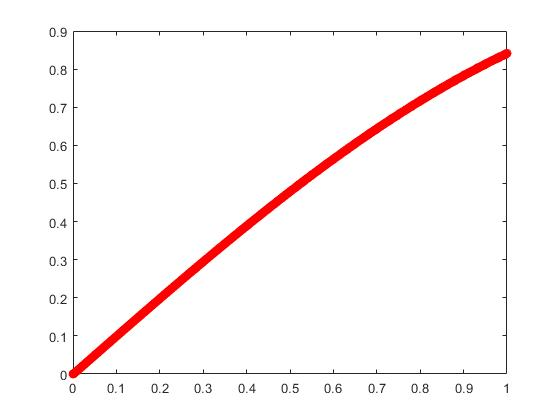
\includegraphics[width=0.9\textwidth]{img/Assignement_7_3.jpg}
                \caption{Figure} 
            \end{figure}
        \subsection{}
            \lstinputlisting[language=Matlab,style=mystyle,caption=Code ]{code/Assignment_7_3_2.m}
            \begin{figure}[H] 
                \centering 
                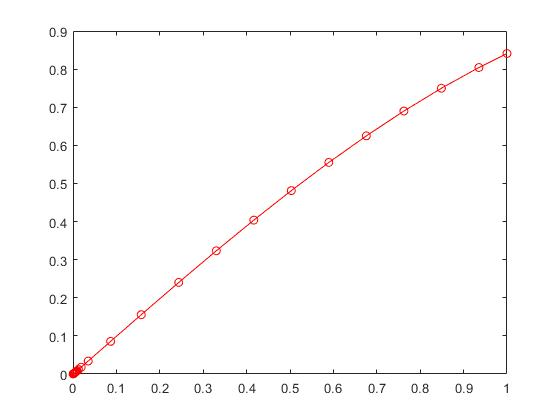
\includegraphics[width=0.9\textwidth]{img/Assignement_7_5.jpg}
                \caption{Figure} 
            \end{figure}
    \section{}
        \subsection{}
            \lstinputlisting[language=Matlab,style=mystyle,caption=Code ]{code/Assignment_7_4_1.m}
        \subsection{}
            \begin{figure}[H] 
                \centering 
                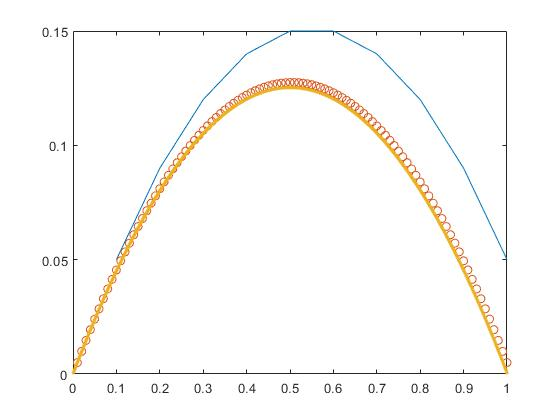
\includegraphics[width=0.9\textwidth]{img/Assignement_7_4.jpg}
                \caption{Figure} 
            \end{figure}
\end{document}